\documentclass[notitlepage]{report}   % list options between brackets

%*****************************
\usepackage{url}
\usepackage{amsmath,amsfonts,amssymb,eucal,eurosym}        
\usepackage{graphicx}
\usepackage{color}
\usepackage[font=small, format=hang, labelfont={sf,bf}, figurename=Fig.]{caption}
\usepackage{cite}
\usepackage{epigraph}
\usepackage[	colorlinks,linkcolor=red,citecolor=red]{hyperref}
%**********************************

\begin{document}

\title{Project No.6\\Comparative Modeling of Protein Structure}
\author{Taylor Kessinger, Zarin Shakibaei, Fabio Zanini}   
\date{18.06.12}
\maketitle

\begin{abstract}
 Modeller is a popular software tool for predicting protein structures using homology modeling~\cite{PROT:PROT340230306}. We use Modeller to predict the structure of a protein sequence by comparing it to a number of protein sequences with known structures. Sequence alignment and structure prediction can both be performed using built-in Modeller classes. We do so, then visualize the result using PyMol~\cite{pymol}. The predicted structure is reasonably close to the true structure of the target.
\end{abstract}

\section*{Introduction}   
Proteins are thus more robust to changes at the sequence level than at the structural level. Evolutionarily, protein structures are much more conserved than protein sequences. Homology modeling exploits this fact by fitting a desired protein sequence with a potentially unknown structure (the target) to any number of similar sequences with known structures (the templates). Given a good alignment between a target and template sequence, a very accurate structure can be predicted. Homology modeling is obviously most successful when the target and template have similar structures.

The goal of this project is to predict the structure of a target, called in the following \texttt{1yje:A}, by using the homology modeling package, Modeller~\cite{PROT:PROT340230306}. As it happens, \texttt{1yje:A} has a known structure in the Protein Database (PDB), so it is possible to check the predicted structure against the experimentally determined one~\cite{flaig1yje}.
 
\section*{Materials and Methods}   
\subsection*{Modeller overview}
Modeller is both a standalone program and a Python package that performs homology modeling by satisfaction of spatial restraints. The basic procedure is the following:
\begin{itemize}
\item The target sequence is aligned against one or more template structures using the sequences and the .pdb file for the templates.
\item Spatial features from the templates, such as dihedral angles, C$_\alpha$-C$_\alpha$ distances, and hydrogen bonds, are determined from the structures of the templates. These are used to derive spatial restraints on the target structure~\cite{sali1994comparative}.
\item A model for the target structure is determined by satisfying these restraints.
\end{itemize}
The following example of a ``spatial restraint" is described in~\cite{sali1994comparative}: if, say, a hydrogen bond to the main chain at a certain residue appears in all or many comparable template structures, it is reasonable to assume that it also appears in the target. In the original implementation of Modeller, ``reasonable to assume'' means that a high probability is placed on this feature appearing in the target structure; probability density functions constraining stereochemistry, main- and side-chain conformations, amd so on are constructed, then combined into a single molecular pdf. Optimizing with respect to this pdf yields the most probable structure given the alignment. The conjugate gradient method is employed by Modeller for this optimization. Here, rather than rely on the molecular pdf, we employ a statistical potential optimized for model assessment, namely DOPE (Discrete Optimized Protein Energy)~\cite{DOPE}.

\subsection*{Initial search}
CS-BLAST, or ``context-specific BLAST''~\cite{csblast}, an improved version of the Basic Local Alignment Search Tool~\cite{BLAST} that takes into account the context of neighboring amino acids in a sequence, was used to find initial matches. Due to the use of context information, CS-BLAST finds a higher number of remotely homologous sequences than BLAST does at a given error rate. A number of hits were returned, namely:
\begin{itemize}
\item The target sequence from the PDB.
\item A number of hits with $e < 0.01$ with reasonable chunks in common with the target sequence.
\item A number of hits with only a domain in common in the middle of the sequence or at the N-terminus. A large gap in $e$-value was visible between the previous hits and these.
\end{itemize}
The CS-BLAST search returned already a multiple sequence alignment (MSA) of the results.

\subsection*{Input data and alignment} 
Efficient general-purpose alignment packages exist, such as MUSCLE~\cite{edgar2004muscle}. In homology modelling, however, the alignment problem is slightly different, because a) only the parts of the proteins that have a well-resolved structure must be used, and b) gap penalities should be weighted by the degree of secondary structure (highly structured regions are more likely to be conserved).

In other words, FASTA files are inappropriate for use with Modeller for two reasons. The first is obvious: Modeller is a homology modeling package, so some information about the structure of template proteins is needed to generate a model. The second is less obvious: A FASTA alignment file does not contain information specifying which positions of the alignment correspond to which residues of the protein. To remedy this, Modeller's modeling capabilities require that input be provided in PIR (Protein Information Resource) format, which contains not only the aligned residues, but an extra comment line specifying the start and end position of the alignment.

To this end, Modeller also contains its own alignment class. Modeller's aligning capabilities include several advantages; for example, gap penalties are lessened outside of secondary structures, based on the argument that secondary structures should be much less robust to insertions and deletions than unstructured parts of the protein. FASTA files can be converted into PIR format by adding the appropriate comment line; this and the PDB files for the template sequences are the minimum requirements needed to generate an alignment. The \texttt{alignment.slign2d()} function allows for a pairwise or multiple sequence alignment and saves the resulting alignment file in PIR format.

\subsection*{Scripting}
Modeller is a command-line only tool, and has no graphical user interface; instead, a script file containing Modeller commands should be provided. Once installed, Modeller can be called from the command line either with the \texttt{mod9.10} command, which automatically calls an bundled Python interpreter (version 2.3) and imports the necessary \texttt{modeller} module, or by locating the Modeller dynamic libraries and importing the module into the current Python interpreter (for this project, version 2.7). If using \texttt{mod9.10}, the name of the desired script can be provided as an argument, and standard output is suppressed and saved to a .log file.

Our program consists of several Python scripts. We chose this design over a single, comprehensive program mostly for reasons of flexibility and platform-independence of the various steps. A brief outline is provided below.
\begin{itemize}
\item \texttt{parse\_blast\_results.py} contains the function \texttt{parse\_blast\_results}, which parses a FASTA file corresponding to our initial alignment and saves the sequence and chain IDs.
\item \texttt{read\_templates.py} contains two functions; \texttt{read\_templates()}, which reads sequence and chain IDs and stores them in a dict, and \texttt{get\_tplname()} returns a typical alignment code name for a template.
\item \texttt{model\_align.py} is a simple alignment test script. It creates a \texttt{environ()} object, which is needed for all Modeller scripts. It then aligns the target, \texttt{1yje:A}, against a random template, \texttt{3tx7:B}. The \texttt{automodel} class is invoked to generate a model pdb file.
\item \texttt{align\_model\_all.py} is an improvement on \texttt{model\_align.py} that produces single alignments of the target against a range of templates, then performs the corresponding predictions.
\item \texttt{model\_align\_multiple.py} generates an MSA of the target and several template sequences-structures. It then invokes the \texttt{automodel} class, which assigns weights to the various templates based on their sequence identity with the target. Three models are generated from the same MSA to evaluate initial-value effects on the result. The \texttt{assess\_methods} option allows DOPE scores to be output to the .log file.
\item \texttt{plot\_figures\_pymol\_multiple.py}, which incorporates the Python structure visualization module \texttt{PyMol} to visualize a .pdb file~\cite{pymol}. It must actually be called from within PyMol and has options to plot the predicted structure against template structures or the true structure, then save either to file.
\end{itemize}

The \texttt{automodel} class offers a wide range of options for incorporating water, disulfide bridges, and a variety of other features, as well as refining only parts of the model. For our purposes, however, most default options sufficed.

Our main script, \texttt{model\_align\_multiple.py}, produces a PDB file with the predicted structure as output. PDB is a standard format, and an example is shown in Fig.~\ref{fig:PDB}

\begin{figure}[h!]
\begin{center}
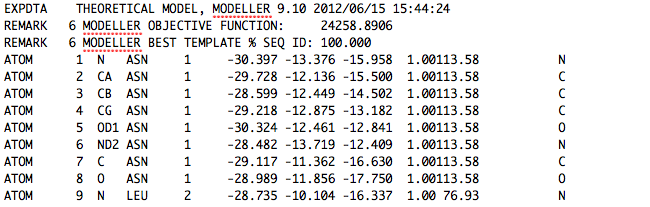
\includegraphics[scale=0.5]{output-15template.png}
 \caption{Sample of a PDB file corresponding to \texttt{1yje:A}, constructed with 15 templates.}
 \label{fig:PDB}
\end{center}
\end{figure}

\subsection*{Visualization}   
Our PyMol script enables us to visualize the .pdb format outputs of our alignment and prediction script and compare it against the known structure of \texttt{1yje:A}. As a sanity check, we can also predict the structure of the target using itself as a template (since \texttt{1yje:A} has a structure in the PDB). Obviously, we expect to see a perfect match in that case, which we do, as can be seen by examining \figurename~\ref{fig:truevtrue}. This confirms that homology modeling is, at least \textit{prima facie}, a sensible approach, and that Modeller does what it claims to do.

\begin{figure}[h!]
\begin{center}
  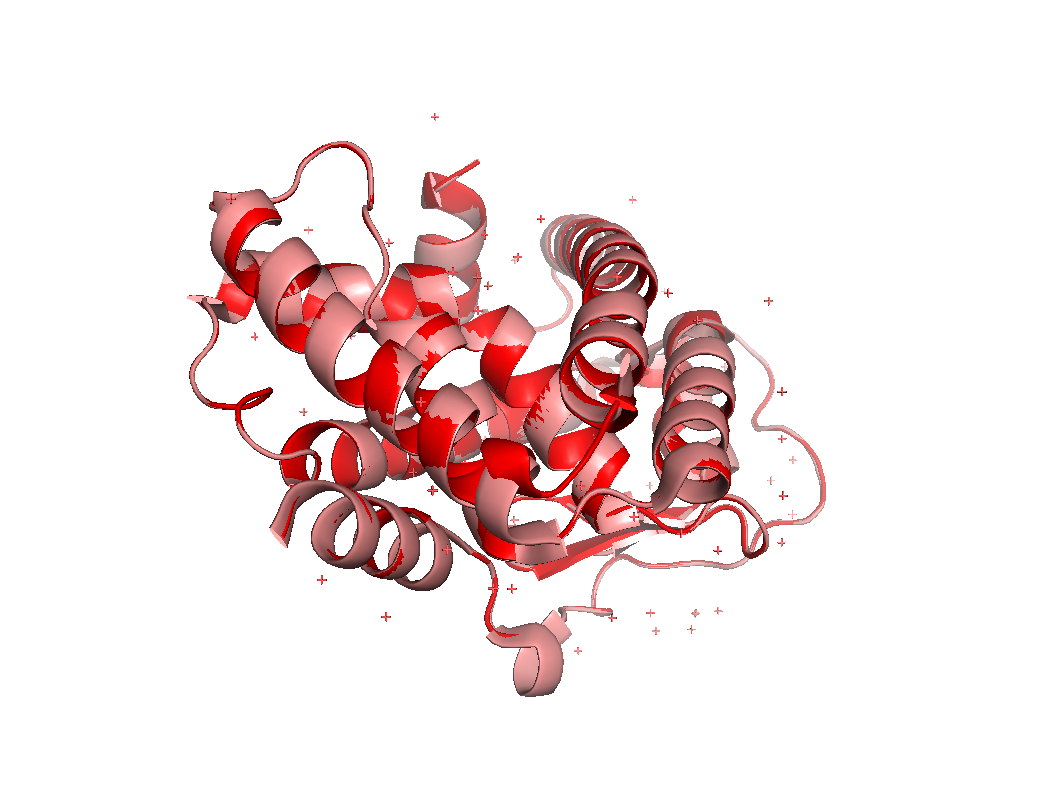
\includegraphics[width=0.8\linewidth]{real_vs_real.png}
\caption{The target threaded onto itself. Colors: red = our model, salmon = true structure.}
\label{fig:truevtrue}
\end{center}
\end{figure}

We also show the results of threading the target onto the top two, top five, and top ten similar PDB entries, as ranked by $e$-value, in \figurename~\ref{fig:tt_2}, \figurename~\ref{fig:tt_5}, and \figurename~\ref{fig:tt_10}. A number of options are available for evaluating the quality of protein models ~\cite{krysh}. Our structures are each selected by generating three multi-template models and selecting the one with the top DOPE score. Notably, introducing the additional entries does not seem to improve the quality of the prediction that much. Even with only two templates, the quality is quite high, however, with only a few small defects, such as the slightly wrong start position for a sheet or helix, are visible.

\begin{figure}[h!]
 \begin{center}
  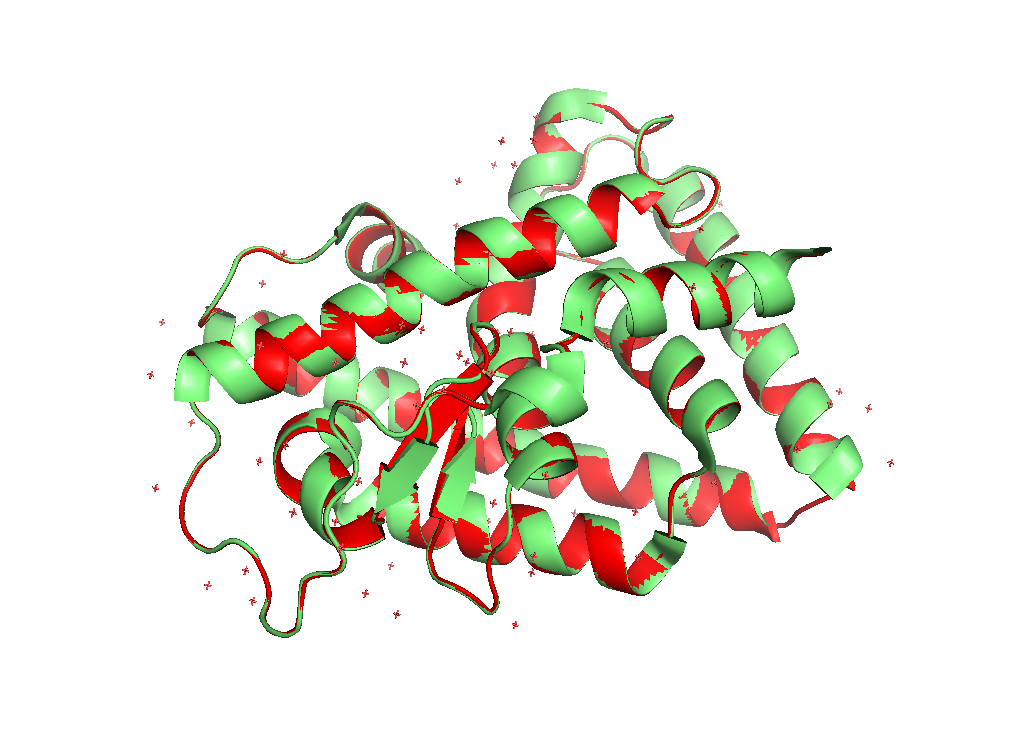
\includegraphics[width=0.45\linewidth]{2_templates_truth.png}
  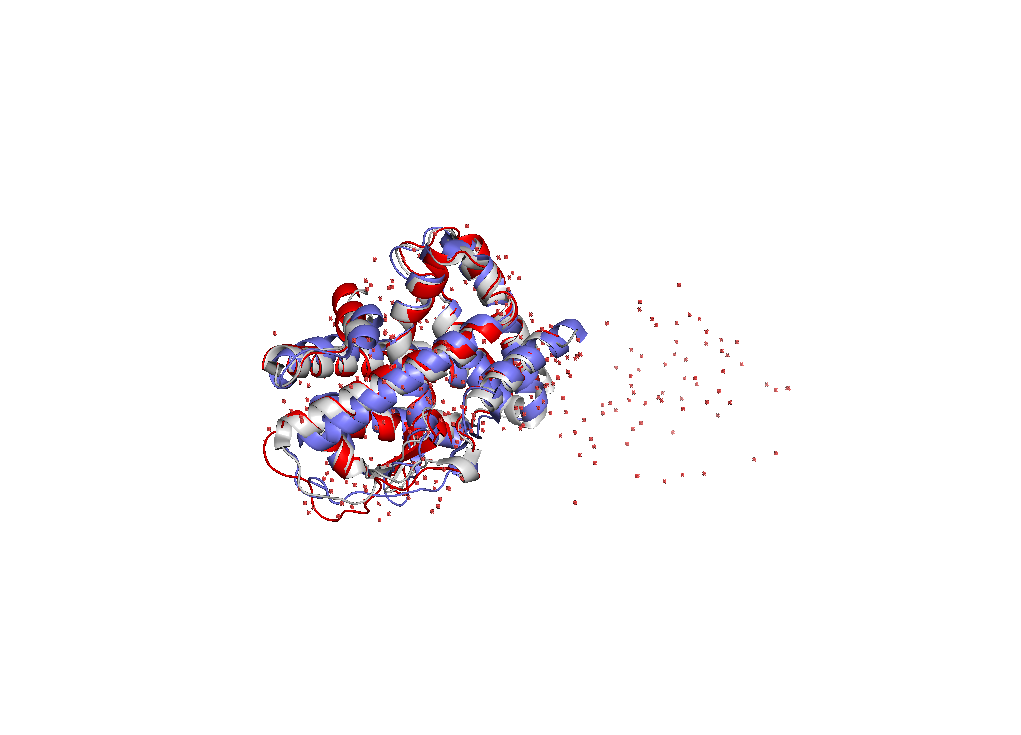
\includegraphics[width=0.45\linewidth]{2_templates.png}
  \caption{A multiple-sequence model: Our unknown sequence threaded onto two similar PDB entries. Left: The predicted structure against the true one. Right: The same against all ten models. Colors: red = our model, green = true structure, other = templates.}
  \label{fig:tt_2}
 \end{center}
\end{figure}


\begin{figure}[h!]
 \begin{center}
  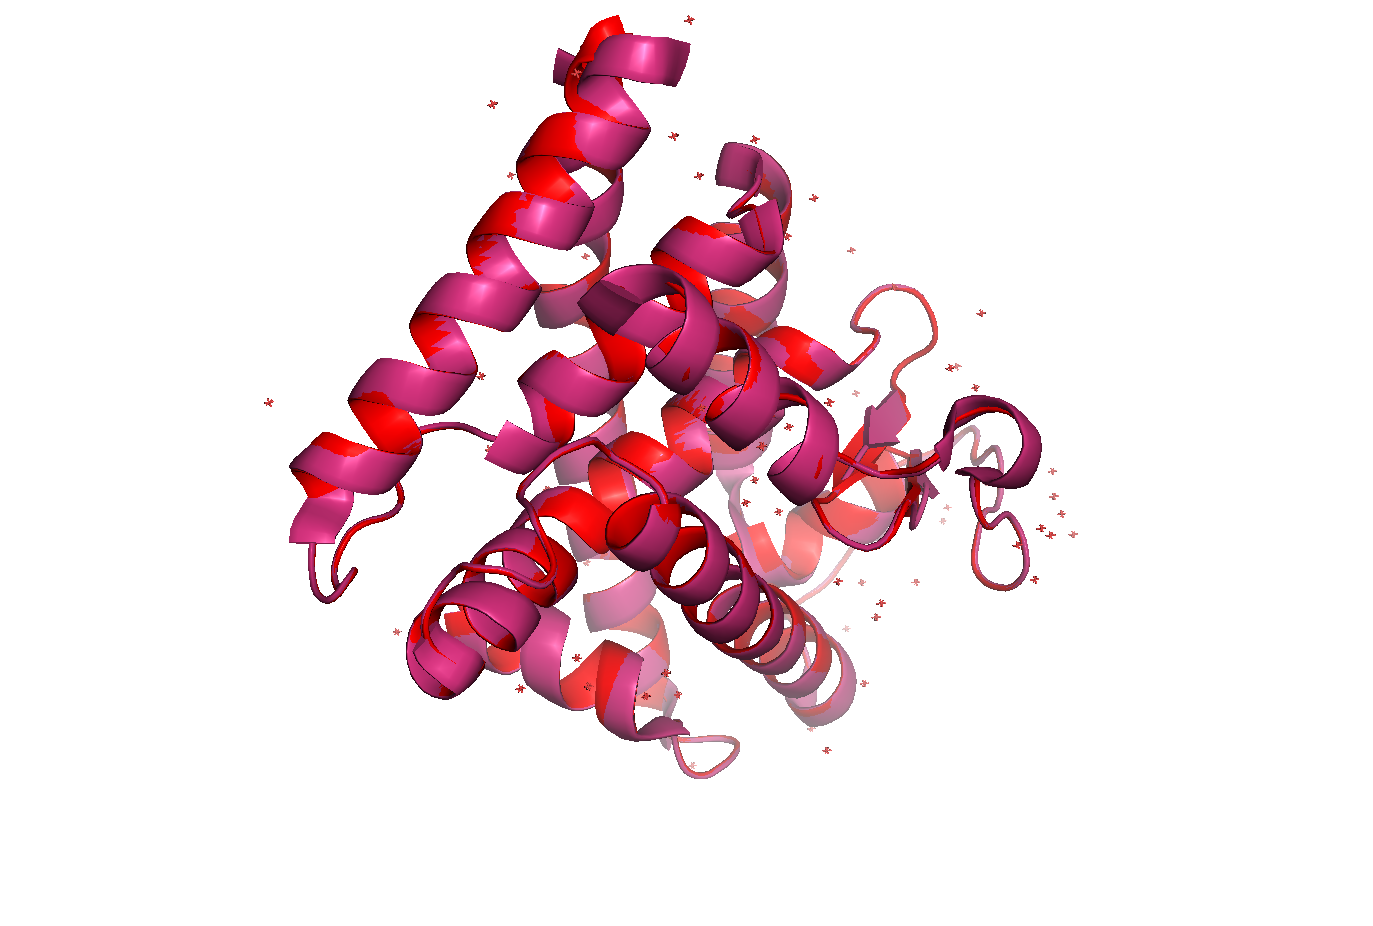
\includegraphics[width=0.45\linewidth]{5_templates_truth.png}
  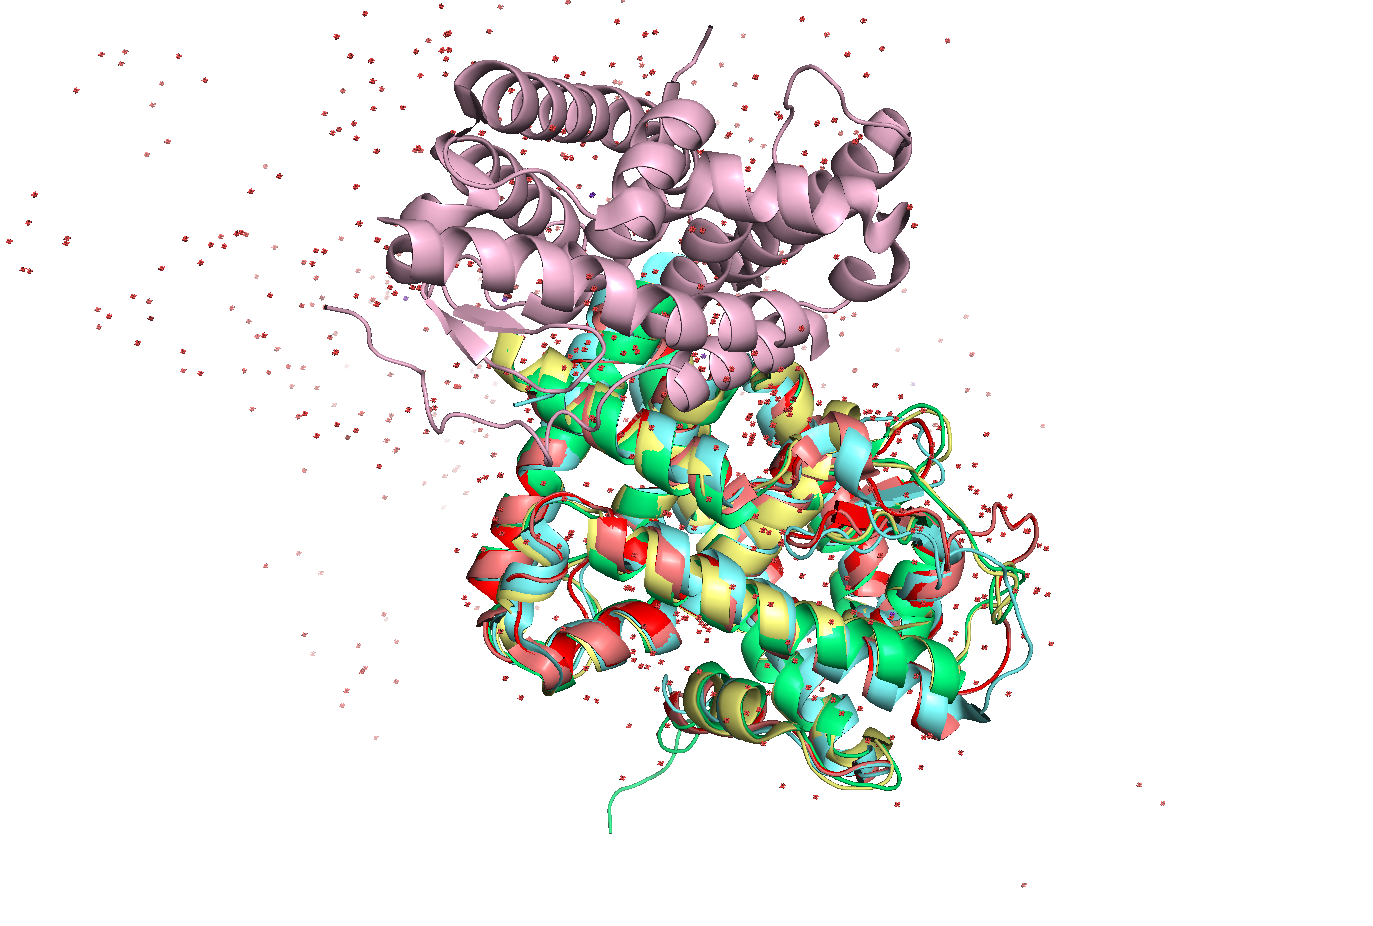
\includegraphics[width=0.45\linewidth]{5_templates.png}
  \caption{A multiple-sequence model: Our unknown sequence threaded onto five similar PDB entries, including ones with lower sequence identity to our target. Left: The predicted structure against the true one. Right: The same against all five models. Colors: red = our model, fuchsia = true structure, other = templates.}
  \label{fig:tt_5}
 \end{center}
\end{figure}

\begin{figure}[h!]
 \begin{center}
  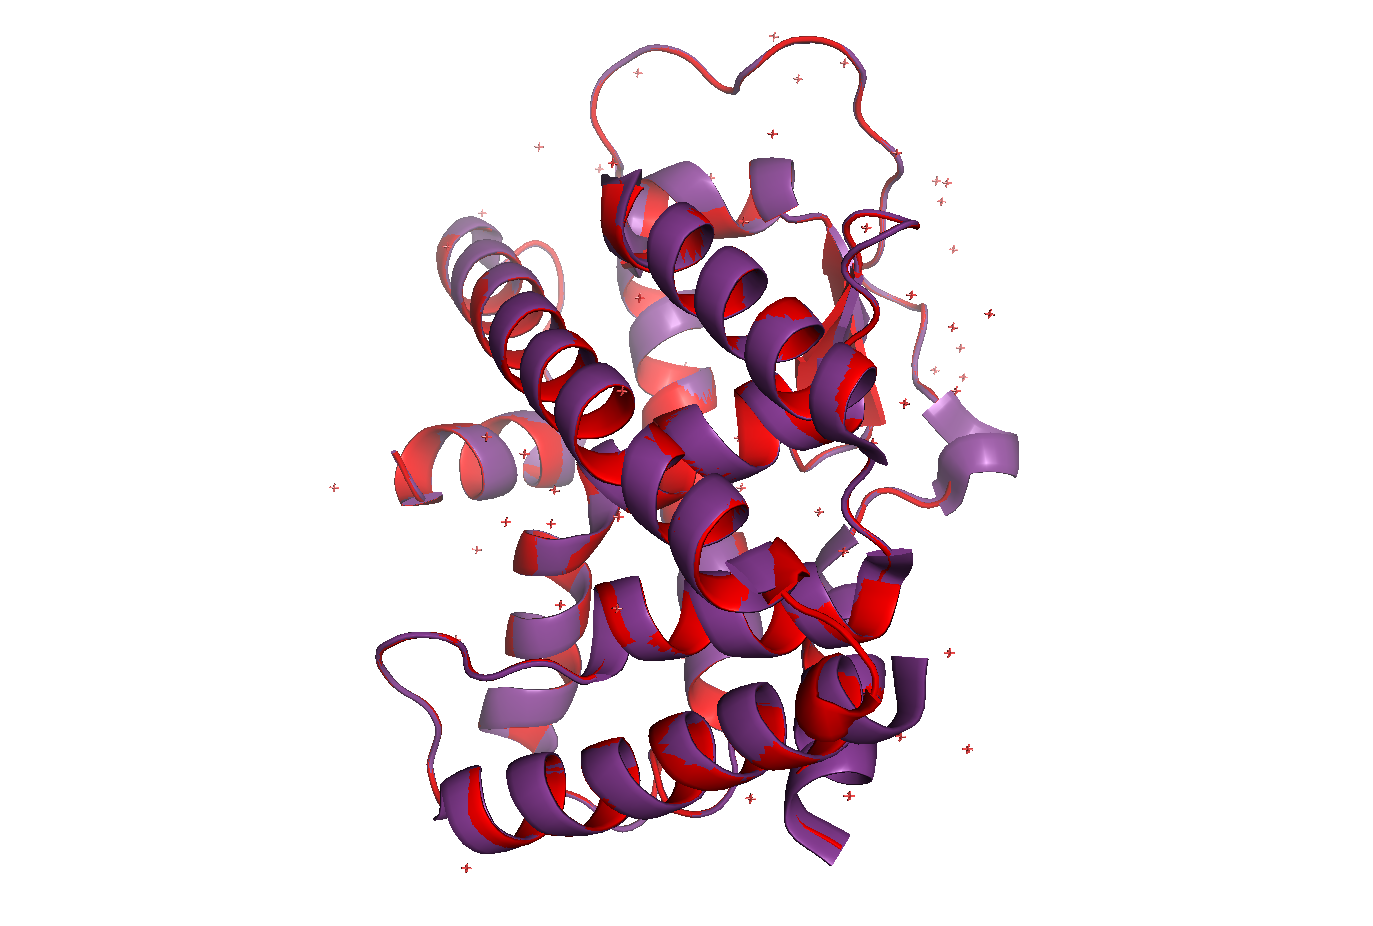
\includegraphics[width=0.45\linewidth]{10_templates_truth.png}
  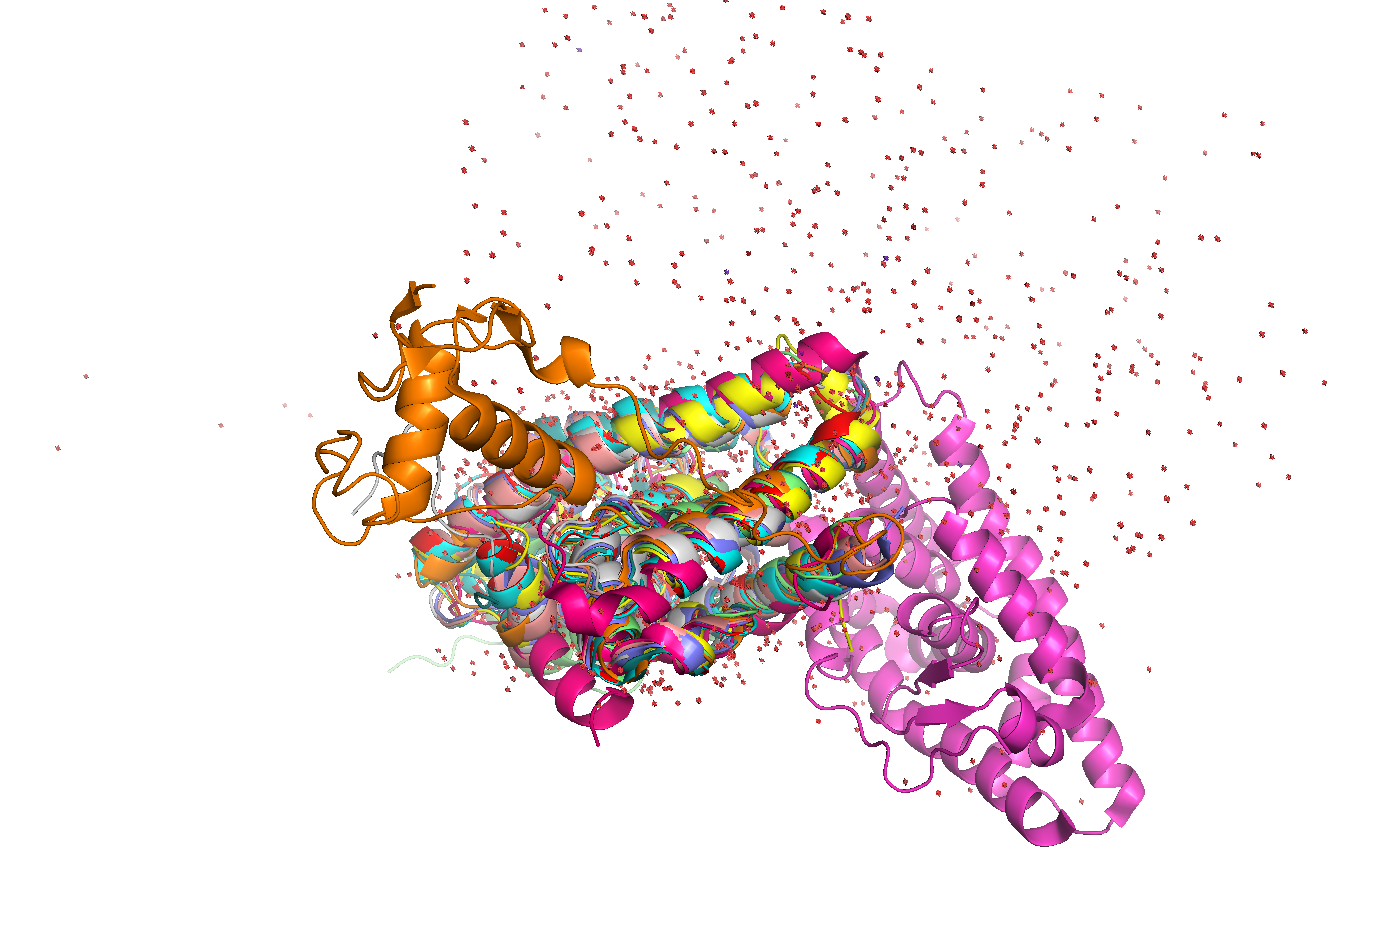
\includegraphics[width=0.45\linewidth]{10_templates.png}
  \caption{A multiple-sequence model: Our unknown sequence threaded onto ten similar PDB entries. Left: The predicted structure against the true one. Right: The same against all ten models. Colors: red = our model, purple = true structure, other = templates.}
  \label{fig:tt_10}
 \end{center}
\end{figure}

In each case, DOPE scores on the order of -30k result, confirming the accuracy of our predictions. Furthermore, the accuracy can be seen visually.

\section*{Discussion}   
Homology modeling is a powerful tool for predicting the structure of unknown proteins. In fact, it has been suggested that the PDB is essentially complete enough to ``solve'' the structure prediction problem, with the only limiting factor being inadequacies in sequence alignment~\cite{zhang2005protein}. This problem, too, may soon be fixed, as tools like CS-BLAST continue to improve the quality and number of hits than can be acquired. Here, we have successfully demonstrated the accuracy of homology modeling when known template structures are available.

One obvious shortcoming of homology modeling is its inability to model proteins that have essentially no homologues. Examples include the venoms of many animals, which are relatively young proteins that are very specific to that particular animal. Since they do not have significant sequence identity with other proteins of known structure, and since structure identity decreases rapidly when sequence identity sinks below about thirty per cent, there is little hope for homology modeling to be effective for these particular proteins.

\section*{Conclusion}   
We have verified the effectiveness of Modeller for predicting the structure of a protein with an unknown sequence. Importantly, the accuracy of our prediction seems to be not terribly sensitive to the number of templates used; even a mere two templates is sufficient enough to generate a very accurate structure, as evaluated both by DOPE score and by visual inspection.

The development version of the source code for this project can be found at \url{https://github.com/tkessinger/bi2-ss12-p6}.

\bibliographystyle{plain}
\bibliography{Project6}

\end{document}
